\documentclass[a4paper]{article}
\usepackage[margin=1in]{geometry} % 设置边距,符合Word设定
%\usepackage{ctex}
\usepackage{lipsum}
\usepackage{cite}
\usepackage{amsmath,amssymb,amsfonts}
\usepackage{algorithmic}
\usepackage{graphicx}
\usepackage{textcomp}
\usepackage{xcolor}
\usepackage{url}
\usepackage{verbatim}
\usepackage[colorlinks=true, allcolors=blue]{hyperref}
\usepackage[section]{placeins}
\usepackage{pdfpages}
\usepackage{indentfirst}

\title{Introduction to AI Coursework}
\author{Runze Yuan 2217498}




\begin{document}

\maketitle

\section{Introduction}

% 说明问题是什么,说明需要哪种算法(回归),说明为什么需要用回归来干这个
\subsection{Question}
% 对于一个发电厂,用它的四个hourly平均环境值来预测其net hourly electrical energy output.

For a Combined Cycle Power Plant, use its hourly average ambient variables to predict the net hourly electrical energy output.

To be specific, the task is to use four input value to predict one output value.

\subsection{Which kind of algorithms to use and why}

Use \textbf{Regression} for the task.

\vspace{5pt}

Reasons:
\begin{itemize}
    \item The aim of regression algorithms is to capture the relationship between inputs and outputs, which is what the task asks for (to predict energy output with four ambient value).
    \item Regression algorithms are capable of predicting future or unseen data.
\end{itemize}

\section{Methods}

\subsection{Algorithms}

In this report I will show results with \textbf{K Neighbors Regressor} and \textbf{Decision Tree Regressor}.

\begin{itemize}
    \item KNR: Find K nearest neighbors in the feature space for the input vector and use the output value of the neighbors to calculate the predicted output.
    \item DTR: DTR builds a decision tree by recursively splitting points into groups based on the result of separation. 
\end{itemize}

\subsection{Metrics}

The Mean Squared Error (MSE), Mean Absolute Error (MAE), and R-squared ($R^2$) are selected as performance metrics for the algorithm. These are common metrics for regression algorithms.

\begin{itemize}
    \item MSE and MAE are metrics that reflects the difference between the predicted result and ground-truth, the lower the better.
    \item $R^2$ reflects the goodness of fitting of the algorithm, and a value close to 1 means a good fit. 
\end{itemize}

\subsection{Baseline}

For the baseline model, use the dummy model in the scikit learn. 

Set all hyperparameters of the dummy to the default value, which means set "parameters" to mean, and both "constants" "quantile" to None.

With these parameters, the dummy model is not an actual regressor and would always output the mean value of the given training output data. 

\subsection{Hyperparameters}


Hyperparameters are parameters that are set prior for models and not changed in the learning process. These parameters control the characteristic of the model and allow adjustments for the user by tuning the hyperparameters.

\begin{itemize}
    \item \textbf{KNR}: In this report I will try to find the optimal \textbf{n\_neighbours}, \textbf{weights}, and \textbf{p}. 
    \begin{itemize}
        \item n\_neighbors: how many nearest neighbors the algorithm use to predict the output value.
        \item weights: changes the weights used in the output generating.
    
        \begin{itemize}
            \item uniform: all nearest neighbors have the same weight.
            \item distance: use distance as weights for the neighbors, distant neighbors have lower weights. 
        \end{itemize}

        \item p: changes the type of distance used in the algorithm
        \begin{itemize}
            \item p=1: apply Manhattan distance for distance calculation.
            \item p=2: apply Euclidean distance for distance calculation. 
        \end{itemize}
        \item other parameters applied but not discussed in this report: 
        \begin{itemize}
            \item algorithm: "auto"
            \item leaf\_size: 30
            \item metric: "minkowski"
            \item metric\_params: "None"
            \item n\_jobs: None
        \end{itemize}
        
    \end{itemize}

    \item \textbf{DTR}: In this report I will try to find the optimal \textbf{max\_depth}, \textbf{min\_samples\_leaf}, and \textbf{splitter}
    \begin{itemize}
        \item max\_depth: the maximum depth of the tree.
        \item min\_samples\_leaf: the minimum sample amount for a node to be a leaf node.
        \item splitter: changes the strategy of splitting samples into different groups in nodes.
        \begin{itemize}
            \item best: evaluate all possible splits and apply the best one which have the best performance.
            \item random: apply the best split among a random generated strategy for randomly selected subsets of the features.
        \end{itemize}
        \item other parameters applied but not discussed in this report: 
        \begin{itemize}
            \item min\_samples\_leaf: 1
            \item min\_weight\_fraction\_leaf: 0.0
            \item max\_features: None
            \item random\_state: 42
            \item max\_leaf\_nodes: None
            \item min\_impurity\_decrease: 0.0
            \item ccp\_alpha: 0.0
        \end{itemize}
    \end{itemize}
\end{itemize}

\subsection{Hyperparameters searching}

\label{sec:HyperparametersSearching}

Use GridSearchCV provided in scikit-learn to search for optimal hyperparameters.

\begin{itemize}
    \item Use 80\% of the provided data as training test in this step, and 20\% for later result verification.
    \item Use 10-fold cross-validation to make sure the hyperparameters show their generalization ability.
    \item Use MSE as metric for hyperparameters performance, because MSE could better illustrate the difference between predicted output and ground-truth.
\end{itemize}

\subsubsection{K Neighbors Regressor}

\begin{itemize}
    \item Preprocess data: Standardize features by removing the mean and scaling to unit variance. Standardizing could make the influence of all features equal.
    \item Search for optimal hyperparameters: Candidates: n\_neighbors = 1$\sim$20, weights = 'uniform', 'distance', p = 1,2    
\end{itemize}

\begin{figure}[htbp]
    \centering
    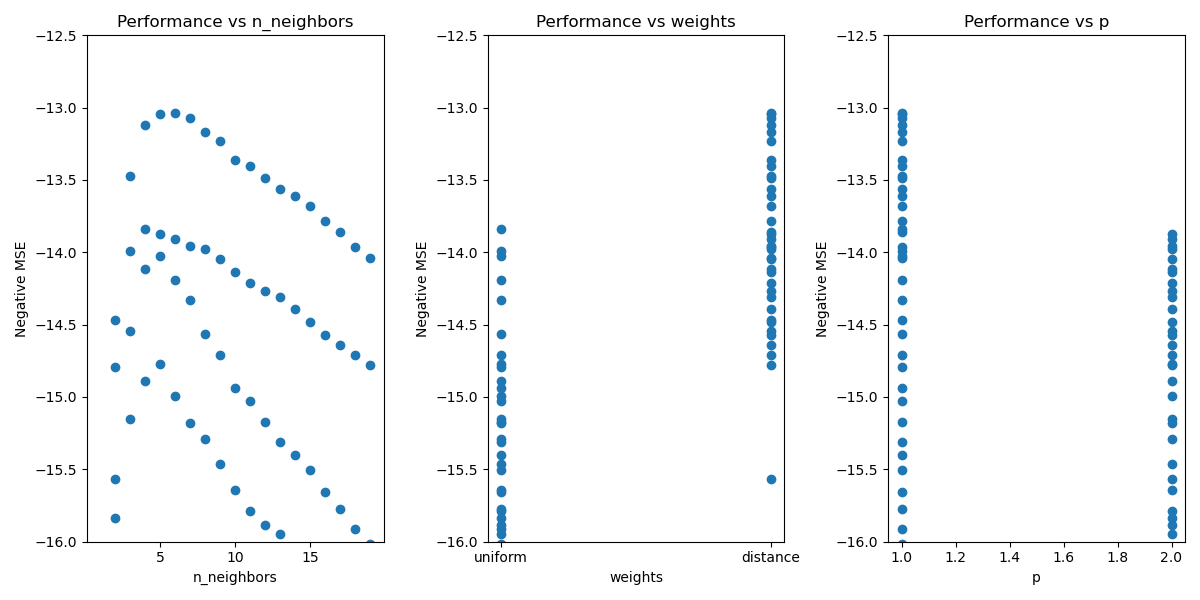
\includegraphics[width = 0.8\linewidth]{Pics/KNR_training.png}
    \caption[]{K Neighbors Regressor hyperparameters searching results. The vertical axis is the negative MSE, with higher values representing better performance.}
    \label{fig:KNR_Searching}
\end{figure}
\FloatBarrier

\textbf{Searching results:}


The performance reaches its peak when the value of n\_neighbors is around 5. Weighting based on distance generally yields better overall performance, and p=1 (Manhattan distance) exhibiting better overall performance.

The optimal hyperparameters found in the searching are: 
\begin{itemize}
    \item n\_neighbors = 7
    \item p = 1
    \item weights = 'distance'
\end{itemize}

and this set of hyperparameters has an MSE of 13.16 on the training data. 


\subsubsection{Decision Tree Regressor}

\begin{itemize}
    \item Search for optimal hyperparameters: Candidates: max\_depth = 5$\sim$20, min\_samples\_leaf = 1$\sim$30, splitter = 'best', 'random'. 
\end{itemize}

\begin{figure}[htbp]
    \centering
    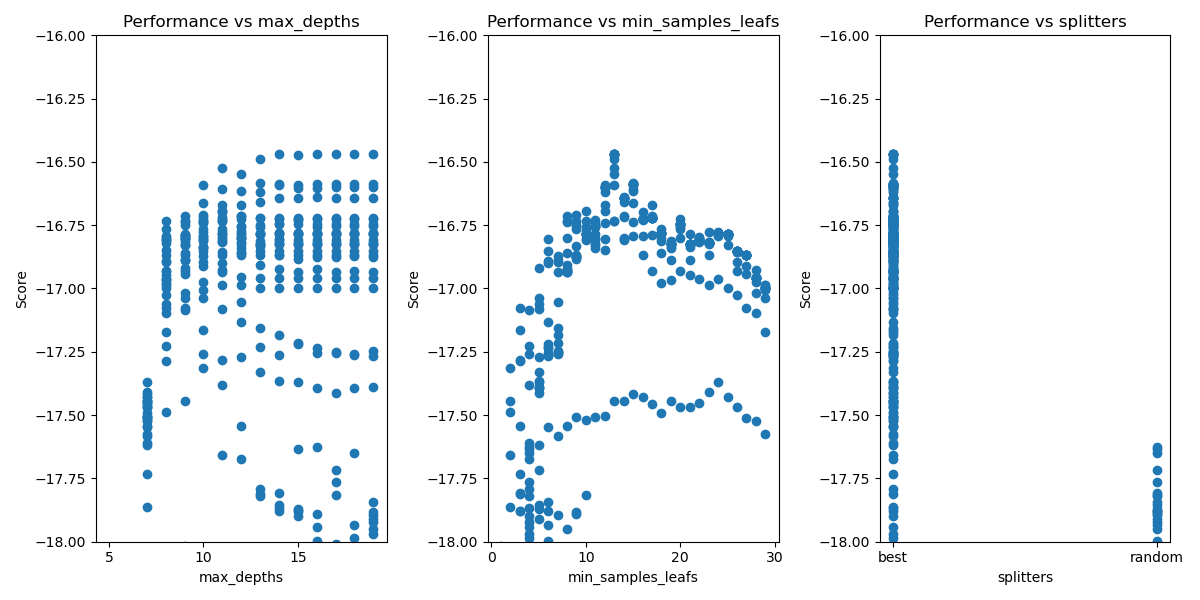
\includegraphics[width = 0.8\linewidth]{Pics/DTR_training.png}
    \caption{Decision Tree Regressor hyperparameters searching results. The vertical axis is the negative MSE, with higher values representing better performance.}
    \label{fig:DTR_training}
\end{figure}

\textbf{Searching results}

The performance reaches its peak when the value of max\_depth is around 15, min\_samples\_leaf is between 10 and 20. Splitter based on the best splitting yields better overall performance.

The optimal hyperparameters found in the searching are: 

\begin{itemize}
    \item max\_depth = 14
    \item min\_samples\_leaf = 13
    \item splitter = "best"
\end{itemize}

and this set of hyperparameters has an MSE of 16.40 on the training data. 

\section{Result and Analysis}

\subsection{Results}

Like previously mentioned in Section \ref{sec:HyperparametersSearching}, the results are performances on the test data which is not used in hyperparameter searching.

Hyperparameters applied are searching results in the previous section.

\begin{table}[htbp]
    \centering
    \begin{tabular}{|l|l|l|l|}
    \hline
    \textbf{Algorithms} & \textbf{MSE} & \textbf{MAE} & \textbf{$R^2$} \\ \hline
    Dummy               & 287.79       & 14.81        & $\approx$ 0           \\ \hline
    K Neighbors         & 12.41        & 2.52         & 0.96        \\ \hline
    Decision Tree       & 16.22        & 2.98         & 0.94        \\ \hline
    \end{tabular}
\end{table}

\subsection{Analysis}

\subsubsection{K Neighbors Regressor}

\begin{itemize}
    \item \textbf{n\_neighbors}: When n\_neighbors is too large, it can lead to a difficulty to capture local pattern due to an excessive number of neighbors. On the other hand, when the value of n\_neighbors is too small, it becomes challenging to capture any patterns effectively (no enough neighbors). In this context, selecting a value of 7  is an optimal trade-off point that strikes a balance.
    \item \textbf{p}: The performance of Manhattan distance and Euclidean distance primarily depends on the dataset. In this case, Manhattan distance (p = 1) exhibits better performance. This may be caused by the patterns in the provided features, like the features have significant difference between each other, or the features are placed on the border of a high dimensional space.
    \item \textbf{weights}: It is normal for weights based on distance have better performance. Distance weighting allows for higher weights to be assigned to more similar points, and suppress the influence of noises in the training data.
\end{itemize}

\subsubsection{Decision Tree Regressor}

\begin{itemize}
    \item \textbf{max\_depth}: An excessively deep decision tree can result in the model being more affected by outliers and noise (overfitting). Additionally, there is a limit to the depth of a decision tree that the dataset can support. Therefore, beyond a certain point, increasing the depth does not improve accuracy. For this dataset, the optimal value for the depth is determined to be 14.
    \item \textbf{min\_samples\_leaf}: A higher value of min\_samples\_leaf can limit the growth of the decision tree and serve as a pruning mechanism, improving generalization and accuracy. However, setting it too high can overly simplify the model and prevent the model from performing detailed classification. For this dataset, the balance point is determined to be 13.
    \item \textbf{splitter}: It is natural for the 'best' splitting strategy to exhibit better performance because it chooses the optimal splitting decisions on every node. The advantage of using the random splitting strategy is that it could generate more efficient decision strategies for complex datasets, but that is at the cost of sacrificing accuracy.
\end{itemize}






\end{document}